\documentclass[12pt]{article}
\usepackage[utf8]{inputenc}
\usepackage{epsfig}
\usepackage{mathrsfs}

%%%%%%%%%%%%%%%%%%%%%%%%%%%%%%%%%%%%%%%%%%%%%%%%%%%%%%%%%%%%%%%%%%%%%%%%
% Reduce margin
%
% \addtolength{\oddsidemargin}{-.85in}
% \addtolength{\evensidemargin}{-.85in}
% \addtolength{\textwidth}{1in}

% \addtolength{\topmargin}{-.85in}
% \addtolength{\textheight}{1in}

% Page format commands:
% Override normal article margins,
% making the margins smaller
\setlength{\textwidth}{6.5in}
% \setlength{\textheight}{9in}
\setlength{\oddsidemargin}{0in}
\setlength{\evensidemargin}{0in}
\setlength{\topmargin}{0.25in}

% \setlength{\parindent}{0pt}
%%%%%%%%%%%%%%%%%%%%%%%%%%%%%%%%%%%%%%%%%%%%%%%%%%%%%%%%%%%%%%%%%%%%%%%%

% hyperlink styling
% use \href{} and \url{}, and colors table of contents links
% use \href{} and \url{}
% \label{sec:name}
% \hyperref[label]{text}
\usepackage{hyperref}
\hypersetup{
    colorlinks=true,
    linkcolor=blue, % was previously black
    filecolor=magenta,
    urlcolor=blue,
    pdftitle={Topological Sweep}
}
\urlstyle{same}
%%%%%%%%%%%%%%%%%%%%%%%%%%%%%%%%%%%%%%%%%%%%%%%%%%%%%%%%%%%%%%%%%%%%%%%%

%%%%%%%%%%%%%%%%%%%%%%%%%%%%%%%%%%%%%%%%%%%%%%%%%%%%%%%%%%%%%%%%%%%%%%%%
% Misc
\usepackage{mathtools}
\usepackage{graphicx} % graphics
\usepackage{enumitem} % listing style (bullet lists)

% add floor and ceiling symbol. Usage: \ceil*{}, \floor*{}
\DeclarePairedDelimiter\ceil{\lceil}{\rceil}
\DeclarePairedDelimiter\floor{\lfloor}{\rfloor}

% A command for primes (')
\newcommand{\p}%
    {\ensuremath{^{\prime}}}

% a command for double primes ('')
\newcommand{\pp}%
    {\ensuremath{^{\prime \prime}}}

% A command for the Kleene star
\newcommand{\str}%
    {\ensuremath{^{\star}}}

% a command for the double star
\newcommand{\sstr}%
    {\ensuremath{^{\star\star}}}
%%%%%%%%%%%%%%%%%%%%%%%%%%%%%%%%%%%%%%%%%%%%%%%%%%%%%%%%%%%%%%%%%%%%%%%%

% \pagestyle {myheadings}
% \markright{TOPOLOGICAL SWEEP}
% \pagenumbering{arabic}
% \title {COMPUTATIONAL GEOMETRY LECTURE NOTES}
% \author{Scribe : Heather Wong}
% \newtheorem{lemma}{Lemma}
% \newtheorem{theorem}{Theorem}
%
% \begin{document}
% \maketitle

\newtheorem{theorem}{Theorem}[section]
\newtheorem{definition}[theorem]{Definition}
\newtheorem{claim}[theorem]{Claim}
\newtheorem{lemma}[theorem]{Lemma}
\newenvironment{proof}{\noindent\bf Proof: \rm}

\newlength{\toppush}
\setlength{\toppush}{2\headheight}
\addtolength{\toppush}{\headsep}


\def\subjnum{Comp 163}
\def\subjname{Computational Geometry}

\def\doheading#1#2#3{\vfill\eject\vspace*{-\toppush}%
  \vbox{
      \hbox to\textwidth{{\bf} \subjnum: \subjname \hfil Professor Diane Souvaine}%
      \hbox to\textwidth{{\bf} Tufts University, Spring 2022 \hfil#3\strut}%
      \hbox to\textwidth{{\bf} \textbf{Topological Sweep} \hfil Editor: Amy Bui}%
    \hrule%
}}

\newcommand{\htitle}[1]{\vspace*{3.25ex plus 1ex minus .2ex}%
\begin{center}
{\large\bf #1}
\end{center}} 

\begin{document}
\doheading{2}{title}{Scribe (2003): Heather Wong}
% \doheading{3}{title}{Editor: Amy Bui}
% \htitle{Topological Sweep}
% \bigskip 
% \bigskip 

%%%%%%%%%%%%%%%%%%

    %%%%%%%%%%%%%%%%%%%%%%%%%%%%%%%%%%%%%%%%%%%%%%%%%%%%%%%%%%%%%%%%%%%%%%%%
    %% Table of Contents
    % \setcounter{tocdepth}{2} 
    % \tableofcontents
    % \pagebreak
    %%%%%%%%%%%%%%%%%%%%%%%%%%%%%%%%%%%%%%%%%%%%%%%%%%%%%%%%%%%%%%%%%%%%%%%%

    \section{Topological sweep: $O(n^2)$ time, $O(n)$ space} %%%%%%%%%%%%%%%%%%%%%%%%%%%%%%%%%%%%%%%%%%%
    \label{sec:topsweep}
        Let $ H $ be a set of $ n $ lines in the plane. Assume that no three
        lines intersect at a point and that none of the lines is vertical.
        Each line intersects $ n-1 $ other lines and thus is divided into $ n
        $ edges. The regions, edges and vertices partition the plane into a
        subdivision known as \underline{arrangement}, or $\mathscr{A}(H)$. If we use a vertical
        sweep line, we need to sort $n^{2} $ intersection points. Whether it
        is possible to sort the $n^{2} $ intersection points determined by $ n
        $ lines in $o(n^{2} \log n) $ is still an open problem.  In
        topological sweep we compromise the straightness of the sweepline to
        acheive better time and space complexities than vertical line sweep.
        The idea of topological sweep is to use a curved line ({\em topological
        line}) with some special properties to simulate a vertical line. Using
        a topological line to sweep the arrangement, we need only $O(n^{2}) $
        time and $O(n) $ space.

        A \underline{topological line} ( \underline{cut} ) is a monotonic line
        in $ y $-direction which intersects every other line exactly once. It
        is specified by a sequence of edges $(c_{1}, c_{2}, , , , , c_{n}) $,
        each contains an intersection point of the cut with a different line in
        the arrangement. Notice that a vertical sweep line runs from $- \infty
        $ to $\infty $ in the $ y $-direction and intersects each line in the
        arrangement exactly once. A cut has the same properties by definition.

        The sweep will be implemented by starting with leftmost cut which
        includes all semi-infinite edges and pushing it to the right till it
        becomes the rightmost cut, in a series of elementary steps.


        An elementary step is performed when the topological line sweeps past
        a vertex of the arrangement. To keep the sweep line a topological
        line, we can only past a vertex which is the intersection point of 2
        consecutive edges in the current cut. (Otherwise, it will intersect
        some line more than once.) Do we always have such a vertex during the
        process of sweeping? That is, will the topological sweep get stuck?

        \begin{lemma}
            \label{lemma.commonendpt}
            There always exist two consecutive edges of the cut with a common
            right endpoint, unless we are considering the rightmost cut.
        \end{lemma}

        \newpage

        \begin{figure}[h]
            \center
            % \includegraphics[width=1\textwidth]{r_endpt.eps}
            \includegraphics[viewport=244 333 371 394]{r_endpt.eps}
            % \epsfig{figure=r_endpt.eps,height=4.5in}
            \caption{The right endpoint of an edge of the cut.}
            \label{figure.r_endpt}
        \end{figure}

        % \vspace{3 in}
        \begin{proof}
            Assume that there are vertices still unprocessed but there is no pair
            of cut edges $c_{k}$, $c_{k+1}$ which share a common right endpoint.
            Let $c_{i}$ be the cut edge with the leftmost right endpoint.  Let
            $c_{j}$ be the edge of the cut on {\it l} which cuts $c_{i}$ at its
            right endpoint $v_{i}$. $c_{j}$s right endpoint ($v_{j}$) is either to the 
            right or to the left of $c_{i}$s right endpoint ($v_i$).  
            See figure \ref{figure.r_endpt}.
                    
            If $v_{j}$ is to the right of $v_{i}$, then the topological line cuts
            {\it l} more than once. So, this can not be the case.

            If $v_{j}$ is to the left of $v_{i}$, then $v_{j}$ is the leftmost
            right endpoint. Contradiction.

            Therefore $v_{i} = v_{j}$. And the leftmost right endpoint is always
            an elementary step.
        \end{proof}
    %%%%%%%%%%%%%%%%%%%%%%%%%%%%%%%%%%%%%%%%%%%%%%%%%%%%%%%%%%%%%%%%%%%%%%%%


    \section{Data Structure} %%%%%%%%%%%%%%%%%%%%%%%%%%%%%%%%%%%%%%%%%%%
    \label{sec:ds}

        \begin{description}
            \item{\textbf{E\big[1:n\big]}} is the array of line equations. $\text{E}[\ i\ ]=(a_{i}, b_{i})$ if the $i^{th}$ line $l_{i}$ of $\mathscr{A}(H)$ is $y=a_{i}x+b_{i}$.
            
            \item{\textbf{HTU\big[1:n\big]}} is an array representing the upper horizon tree. $\text{HTU}[\ i\ ]$ is a pair $(\lambda_{i}, \rho_{i})$ of indices indicating the lines that delimit the segment of $l_{i}$ in upper horizon tree to the left and to the right, respectively. If this segment is the leftmost on line $l_i$, we set $\lambda_i = -1$; if it is the rightmist $l_i$, we set $\rho_i = 0$.

            \item{\textbf{HTL\big[1:n\big]}} represents the lower horizon tree and is defined similarly.

            \item{\textbf{I}} is a set of integers, represented as a stack. If $i$ is in I, then $c_{i}$ and $c_{i+1}$ share a common right endpoint.
            

            \item{\textbf{M\big[1:n\big]}} is an array holding the current sequence of indices that from the lines $m_{1}$, $m_{2}$,  ,  ,  ,  , $m_{n}$ of the cut.
            
            \item{\textbf{N\big[1:n\big]}} is a list of pairs of indices indicating the lines delimiting each edge of the cut.

        \end{description}


        \pagebreak

        The {\em upper horizon tree} of a cut is constructed by starting with the
        cut-edges and extending them to the right. When two edges come together
        at an intersection point, only the one of higher slope continues to the
        right. 
        
        % If the segment of l$_{i}$ in HTU is the leftmost on l$_{i}$,
        % then $\lambda_{i}= -1$, if it is the rightmost then $\rho_{i}=0$.  See figure \ref{figure.upperlower}.

        The {\em Lower horizon tree} is constructed similarly.  The difference is
        that when two edges intersect, only the one of lower slope continues
        to the right. See figure \ref{figure.upperlower}.

        Given HTU and HTL, the right endpoint of the edge on $l_{i}$ is
        identified by the closer of HTU[$i$] and HTL[$i$].

        \begin{figure}
            \center
            \includegraphics[viewport=239 310 369 388]{upperlower_HT.eps}
            %[height=2in]{upper_HT.eps}
            %\epsfig{figure=upper_HT.eps,height=3in}
            \caption{Upper and Lower Horizon Trees}
            \label{figure.upperlower}
        \end{figure}
    \newpage
    %%%%%%%%%%%%%%%%%%%%%%%%%%%%%%%%%%%%%%%%%%%%%%%%%%%%%%%%%%%%%%%%%%%%%%%%


        \section{Example Arrangement and Cut} %%%%%%%%%%%%%%%%%%%%%%%%%%%%%%%%
        \label{sec:example}

        Figure \ref{figure.linecut} contains a modified $\mathscr{A}(H)$ from \cite{edel1989} with a topological line and the associaed cut. Figure \ref{figure.uht} and \ref{figure.lht} are the respective upper and lower horizon trees. \\ 

        The Data structures are defined below for the arragement in Figure \ref{figure.linecut}, \ref{figure.uht}, and \ref{figure.lht}. \\


        \begin{tabular}{rrcrrcrr}
            E:  & $(a_1, b_1)$ &    & HTU:  & $(-1, 2)$ &  & HTL: & $(-1, 0)$ \\ 
                & $(a_2, b_2)$ &    &       & $(-1, 5)$ & &       & $(-1, 1)$\\
                & $(a_3, b_3)$ &    &       & $(5,  4)$ & &       & $(5,  1)$\\
                & $(a_4, b_4)$ &    &       & $(5,  0)$ & &       & $(5,  3)$\\
                & $(a_5, b_5)$ &    &       & $(3,  0)$ & &       & $(3,  1)$\\
                & Fig. \ref{figure.linecut} & & & Figure \ref{figure.uht} & & & Figure \ref{figure.lht} \\
            & & & & & & & \\
            \hline
            & & & & & & & \\
            I:  & 4            &    & M:    & 1         &  & N:   & $(-1, 2)$\\
                & 1            &    &       & 2         &  &      & $(-1, 1)$\\
                &              &    &       & 5         &  &      & $(5,  4)$\\
                &              &    &       & 3         &  &      & $(5,  3)$\\
                &              &    &       & 4         &  &      & $(3,  1)$ \\
                & Figure \ref{figure.linecut} & & & Figure \ref{figure.uht}, \ref{figure.lht} & & & Figure \ref{figure.linecut}
        \end{tabular}

        

        
        \begin{figure}
            \center
            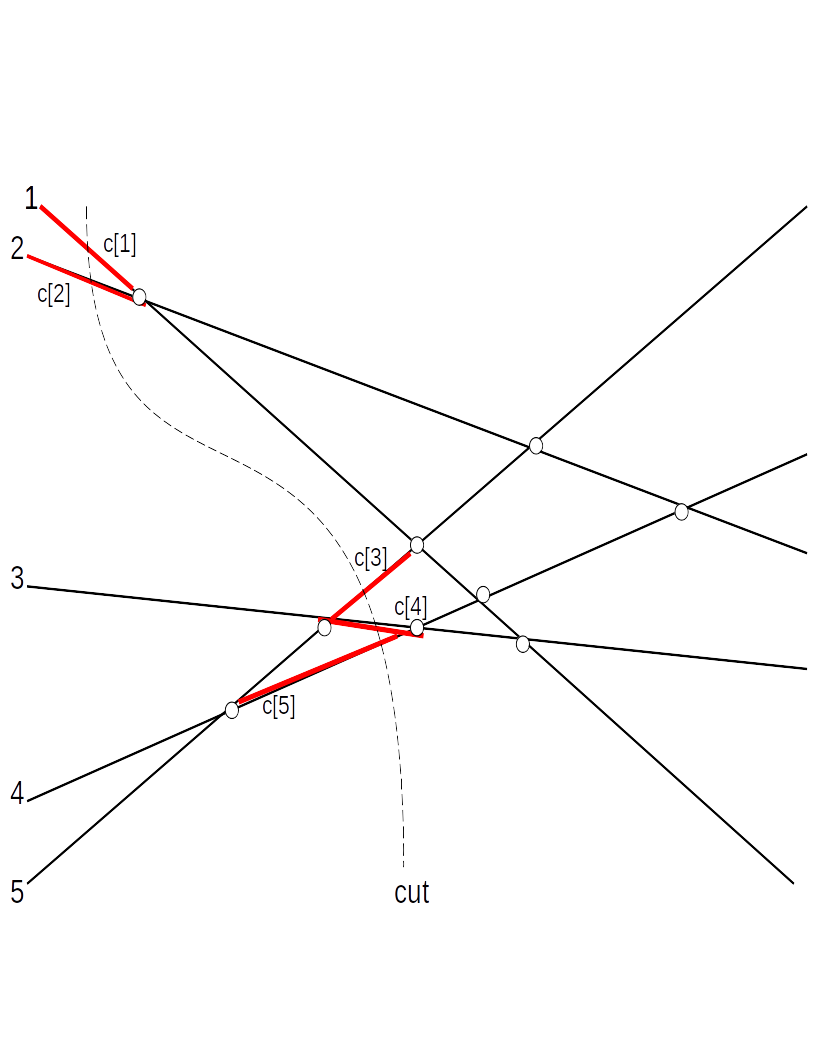
\includegraphics[width=0.7\textwidth]{linecut.png}
            \caption{topological line with associated cut, modified from Edelsbrunner, Guibas (1989)}
            \label{figure.linecut}
        \end{figure}

        \begin{figure}
            \center
            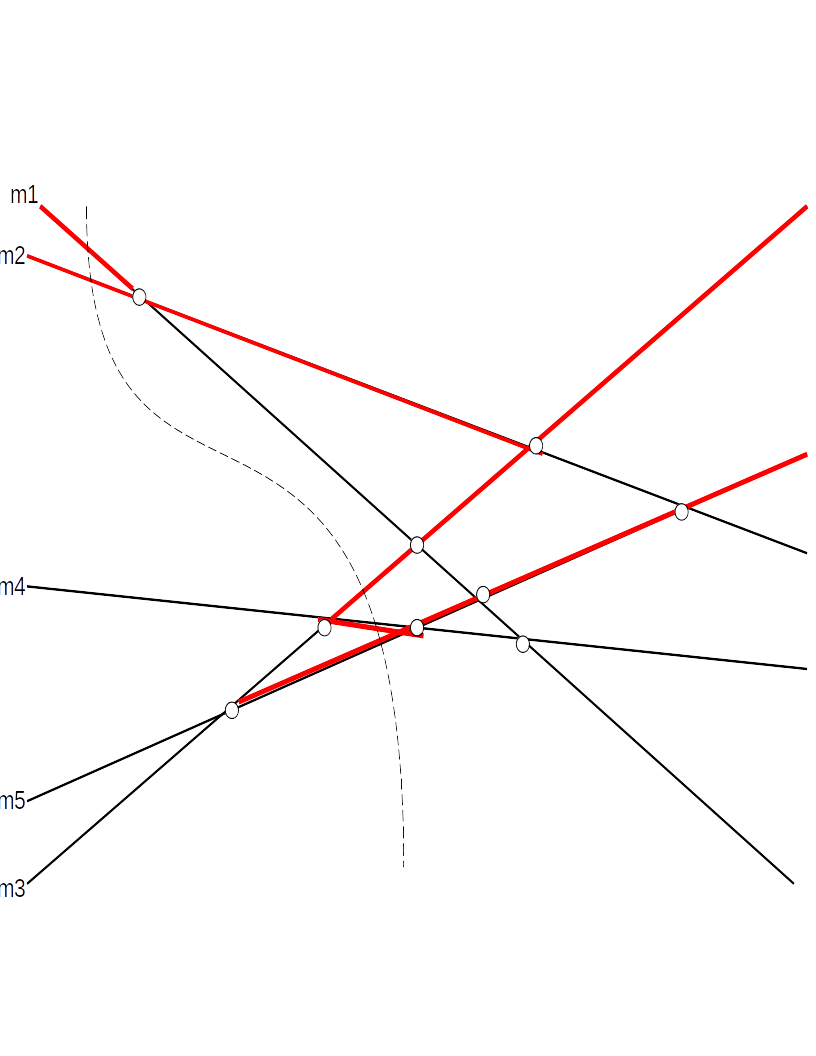
\includegraphics[width=0.7\textwidth]{uht.png}
            \caption{upper horizon tree, modified from Edelsbrunner, Guibas (1989)}
            \label{figure.uht}
        \end{figure}

        \begin{figure}
            \center
            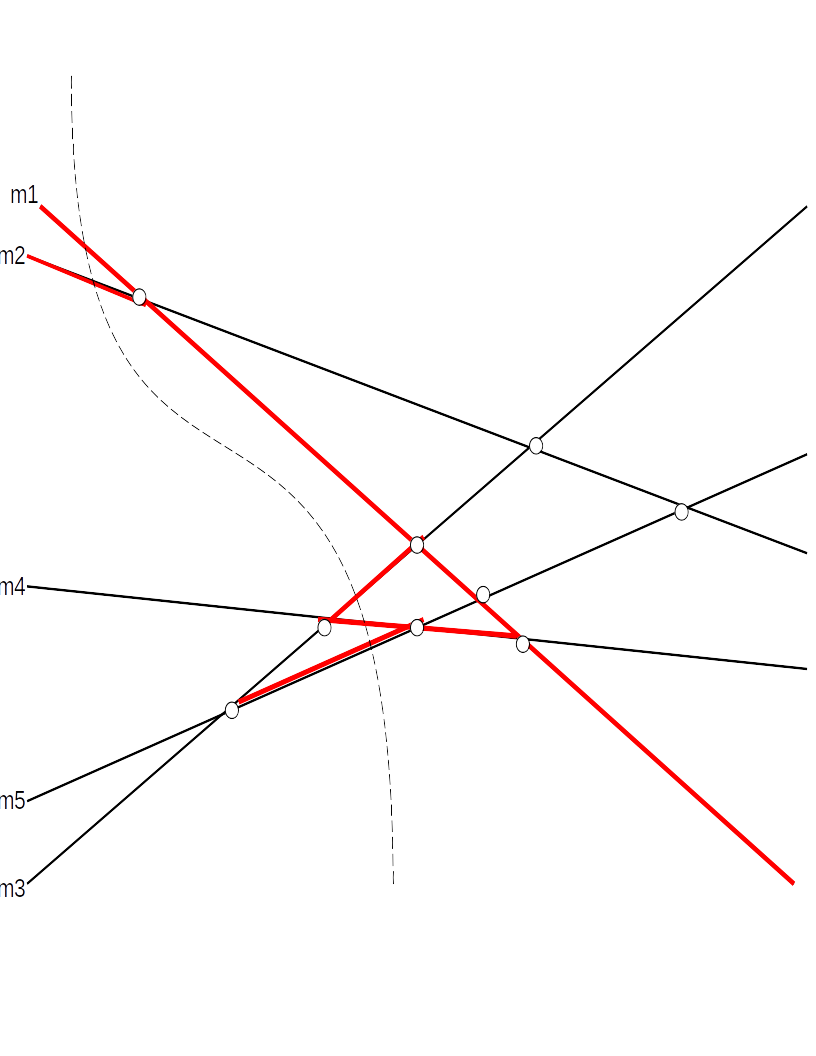
\includegraphics[width=0.7\textwidth]{lht.png}
            \caption{lower horizon tree, modified from Edelsbrunner, Guibas (1989)}
            \label{figure.lht}
        \end{figure}

        \newpage
    %%%%%%%%%%%%%%%%%%%%%%%%%%%%%%%%%%%%%%%%%%%%%%%%%%%%%%%%%%%%%%%%%%%%%%%%

%\newpage
%\begin{figure}
%\center
%\includegraphics[viewport=239 310 369 388]{lower_HT.eps}
%\epsfig{figure=lower_HT.eps,height=3in}
%\caption{Lower Horizon Tree}
%\label{figure.lower}
%\end{figure}

        \section{The algorithm} %%%%%%%%%%%%%%%%%%%%%%%%%%%%%%%%%%%%%%%%%%%
        \label{sec:algo}

        {\bf Initialization:}

        \begin{enumerate}
            \item  Sort the lines of the arrangement by slope.
            \item  Find the leftmost and the rightmost intersection point of the
                lines.
                Let the two points be $(x_{l},y_{l})$ and $(x_{r},y_{r})$.
            \item Create vertical lines $x = x_{l} - 1 , x = x_{r} + 1 $ as left
                boundary and right boundary.
                Determine the intersection points of  lines $l_{1}, , , l_{n}$
                with the boundaries.
            \item Create upper horizon tree:\\
                Insert $l_{1}, , , l_{n}$ in order to make a ``hammock'': \\
                Assume $l_{1}, , , l_{k}$ have been inserted. These lines form
                an {\em upper bay} as shown in figure \ref{figure.init}. To insert
                $l_{k+1}$, begin at its endpoint on the left boundary. Walk in
                counter clockwise order around the bay till we find the
                intersection point of $l_{k+1}$ with an edge.
            \item Create lower horizon tree similarly by starting the travers at
                endpoints on the right boundary.
            \item Initialize N:
                Let HTU[i] = ( -1, $r$ ) and HTL[i] = ( -1, $s$).  If $l_{r}$
                intersects $l_{i}$ to the left of the intersection point of
                $l_{s}$ and $l_{i}$ then the right delimiting line of $e_{i}$
                is r. Otherwise, the right delimiting line of $e_{i}$ is s.
            \item Initialize I by scanning N.
        \end{enumerate}


        \begin{figure}
            \center
            \includegraphics[viewport=265 328 348 390]{initialization.eps}
            %\epsfig{figure=initialization.eps,width=4in}
            \caption{Creating a hammock.}
            \label{figure.init}
        \end{figure}

        Step 1 takes $O(n\log n)$ time. Step 2 could be done in linear time
        since the leftmost and rightmost intersection points must be the 
        intersection points of two consective lines in the sorted order. Step
        3,6,7 take linear time. 

        Now lets look at step 4. When inserting line $l_{i}$, each edge on the
        bay will be traversed once. There are $O(n)$ edges on the bay and
        there are $ n $ lines to be inserted. So we have $O(n^2)$. Could we
        find a tighter bound? Notice that our lines are inserted in decreasing
        order of slopes. Edges on the bay that fail to intersect with line
        $l_{i}$ will not appear on the new bay formed after we insert line
        $l_{i}$. Each line can only fail once, and therefore be traversed once.
        So, HTU can be created in $O(n)$ time.

        By similar argument, step 5 also takes $O(n)$. Hence, the initialization
        can be done in $O(n)$ after sorting of lines.

        \vspace{.2 cm}

        {\bf Elementary Step}

        \vspace{.2 cm}

        After initialization, a series of elementary steps has to be executed.
        Notice that when passing a valid vertex (stored in I), only the two
        cut edges involved get changes, all other edges remain the same.

        \vspace{.2 cm}

        While I$\neq \Lambda$
        \begin{enumerate}
            \item Pop $i$ from I
            \item Swap M[$i$], M[$i+1$] /*lines are going to cross, after the elementary step*/
            \item N[$i].\lambda \leftarrow$ N[$i+1].\rho $ \\
                N[$i+1].\lambda \leftarrow$ N[$i].\rho $ /*the point of elementary step
            becomes the left endpoint of the two new cut edges */ 
            \item Update HTU, HTL.
            \item N[$i].\rho \leftarrow $ closer {HTU[M($i)].\rho$,HTL[M($i)].\rho$} \\
                N[$i+1].\rho \leftarrow$ closer {HTU[M($i+1)].\rho$,HTL[M($i+1)].\rho$} \\
                /* find the new right endpoints */
            \item If N[$i+1].\rho =$ M[$i+2$] then push $i+1$ into I. \\
                If N[$i].\rho =$ M[$i-1$] then push $i-1$ into I. \\
                /* push valid vertices formed after sweeping into I if there is any */
        \end{enumerate}

        The steps 1,2,3,5,6 require just O(1) time. Lets take a look at step 5.

%\newpage
%\vspace{4in}

        \begin{figure}
            \center
            \includegraphics[viewport=205 290 401 426]{update_htu.eps}
            %\epsfig{figure=update_htu.eps,width=5in}
            \caption{Updating the Horizon Tree}
            \label{figure.update_htu}
        \end{figure}

        \vspace{.2 cm}

        {\bf Update HTU}

        \vspace{.2 cm}

        Assume that an elementary step is done after passing point $E$, which
        is the common right endpoint of edge $c_{i}$ and $c_{i+1}$. Let
        $s_{i}$ and $s_{i+1}$ be the left endpoints of $c_{i}$ and $c_{i+1}$
        respectively. At first, HTU[M[$i$]] contains the segment ${\overline{ 
        s_{i}E}}$ and HTU[M[$i+1$]] conatins the segment
        ${\overline{s_{i+1}P}}$.
        After sweeping over $E$, HTU[M[$i$]] should contain ${\overline{EP}}$
        and HTU[M[$i+1$]] should contain ${\overline{EQ}}$. All other entries
        of HTU remain the same.  Updating HTU[M[$i$]] takes only constant time
        since we already have $E$ and $P$. To update HTU[M[$i+1$]], we need to
        traverse the bay till line $l_{M[i]}$ hits the bay.  See figure \ref{figure.update_htu}.

        To see the time complexity, consider the following charging system:
        For each edge traversed, we charge a unit cost to the node $x$
        corresponding to the elementary step. If some where later, an
        elementary step at node $z$ makes the edge that charges $x$ invisible
        from $x$, then we'll transfer the one unit charge to node $z$.

        \newpage

        For example, consider the arrangement in figure \ref{figure.elem_step}. First there
        is an elementary step at $x$, which modified the corresponding HTU
        entries from ${\overline{qt}}$ and ${\overline{px}}$ to ${\overline{xt}}$
        and ${\overline{xu}}$ respectively. So, each of edge $a,b,c$ and $d$
        charge one unit to $x$. Next elementary step occurs at point $y$,
        which changes the involving HTU entries from ${\overline{xt}}$ and
        ${\overline{ry}}$ to ${\overline{yt}}$ and ${\overline{yz}}$.  Finally,
        the elementary step at point $z$ changes HTU entries from ${\overline{
        xu}}$, ${\overline{yz}}$ to ${\overline{zu}}$ and ${\overline{zv}}$. The
        newly created edge ${\overline zv}$ makes edge $d$ invisible from node
        $x$, the charge due to traversing $d$ is transferred from node $x$ to
        node $z$.  %See figure \ref{figure.elem_step}.


        \begin{figure}
            \center
            \includegraphics[viewport=181 282 427 449]{elem_step.eps}
            %\epsfig{figure=elem_step.eps,height=4in}%,width=5in}
            \caption{The elementary step at z creates edge zv, making x invisible from d.}
            \label{figure.elem_step}
        \end{figure}

        \begin{lemma}
            \label{lemma.vertexcharge}
            At the end of the algorithm each vertex is charged at most once for
            every edge on an incident region for the HTU ( HTL ) computation.
        \end{lemma}

        \begin{proof} A vertex $v$ is charged only during the excecution of the
        elementary step at $v$. It gets one charge for every edge traversed,
        each of which is currently visible from it. It also gets one charge
        for each edge of the same region that is seperated by the current edge
        from its old vertex. If sometime later, an elementary step makes the
        edge invisible from $v$, then this edge will not be in the same region
        with $v$ and the charge of the edge will be transferred to some other
        vertex. So, at the end of the algorithm, only the edges that is in the
        incident region of $v$ will charge $v$ and each of them can charge $v$
        at most once.
        \end{proof}

        \begin{lemma}
            \label{lemma.charge1}
                    $\sum_{R \in l}^{ } \mid R \mid = O(n)$.
        \end{lemma}

        \begin{proof} The idea of this proof is to charge each edge of the
        faces that touch $l$ to vertices on $l$ and bound the number of
        charges of each vertex. Since the number of vertices on $l$ is $O(n)$,
        we have   $\sum_{R \in l}^{ } \mid R \mid = O( c * n) = O(n)$.

        Let $l(e_{i})$ denotes the line that contains edge $e_{i}$. Consider
        the following charging system: \\

        For each face $F$ adjacent to line $l$ and above $l$

        \hspace{.2in} For each edge $e_{i}$ arranged in counter clockwise
        order except the ones

        \hspace{.6in} touching $l$ 

        \hspace{.4in} If $l(e_{i})$ intersects $l$ to the left of $F$

        \hspace{.4in} then charge one cost to the intersection point of
        $l(e_{i-1})$ with $l$

        \hspace{.4in} else charge one cost to the intersection point of
        $l(e_{i+1})$ with $l$\\

        For example, in figure \ref{figure.charges}, $P_{1}$ gets 2 charges, one from
        edge $d$, one from edge $r$. $P_{2}$ gets 2 charges from $c$ and $s$.
        $P_{3}$ gets one charge from $b$, etc.

        \begin{figure}
            \center
            \includegraphics[viewport=185 252 412 420]{charges.eps}
            %\epsfig{figure=charges.eps,width=4.8in}
            \caption{Edge Charges}
            \label{figure.charges}
        \end{figure}

        Similarly, for each face below $l$, we charge the vertices on $l$ in
        the similar way. For each vertex of $l$, the number of charges it gets
        is less than or equal to 4 - 2 from edges of the face above $l$, and 2
        from those below $l$. Therefore, there are $O(n)$ edges that get
        charges.

        Now, let's see the edges that don't get any charge: For each vertex
        $v$ on $l$, there are two edges that have $v$ as its right or left
        endpoint and don't get any charge (for example, edges $a$ and $g$ in
        the figure). Also, the edges that lie on $l$ do not get any charge
        either.  There are $O(2n+n) = O(n)$ such edges altogether.

        So, $\sum_{R \in l}^{ } \mid R \mid = O(4n+2n+n) = O(n)$.
        \end{proof}

        \begin{lemma}
        \label{lemma.charge2}
                $\sum_{R \in H}^{ } \mid R \mid ^{2} = O(n^{2})$.
        \end{lemma}

        \begin{proof}   $\sum_{l \in H}^{ } \sum_{R \in l}^{ } \mid R \mid =O(n^{2})$ and \\
        $O(n^{2}) = \sum_{R \in H}^{ } \mid R \mid ^{2}$ from \ref{lemma.charge1}.
        \end{proof}

        \begin{theorem}
            The total cost of updating HTU (or HTL) through all the elementary
            steps is O($n^2$). 
        \end{theorem}

        \begin{proof} From lemma \ref{lemma.vertexcharge} we know that an edge $e$ charges a vertex
            only if they are in the same region and may do so only once. Consider
            region $R$ in the arrangement. Each of its vertices can get at most
            $\mid R \mid$ charges, and there are $\mid R \mid$ vertices in $R$.
            So, there are at most $\mid R \mid ^{2}$ charges associate with $R$.
            Summing this over all regions we get $\sum_{R \in H}^{ } \mid R \mid
            ^{2} = O(n^{2})$ by lemma \ref{lemma.charge2}.

            \vspace{.2cm}
            Hence all the topological sweep can be carried out in O$(n^2)$ time.
            As for the space requirement, all the data structures maintained (6
            arrays) are of linear size. So, space requirement is $O(n)$.
        \end{proof}
    %%%%%%%%%%%%%%%%%%%%%%%%%%%%%%%%%%%%%%%%%%%%%%%%%%%%%%%%%%%%%%%%%%%%%%%%



    %%%%%%%%%%%%%%%%%%%%%%%%%%%%%%%%%%%%%%%%%%%%%%%%%%%%%%%%%%%%%%%%%%%%%%%%
    %% Reference
    \begin{thebibliography}{1}
        \bibitem[1]{edel1989}H. Edelsbrunner and  L.J. Guibas, \href{https://www.sciencedirect.com/science/article/pii/002200008990038X}{Topologically Sweeping an Arrangement}. {\it J. of Computer and System Sciences}, 38:165-194, 1989
        \bibitem[2]{dobsouv}D. Dobkin and D. L. Souvaine, "Computational Geometry - A User's Guide", Chapter 2 of {\it Algorithmic and Geometric Aspects of Robotics}, J.T.Schwartz and C.K.Yap.
        \bibitem[3]{notes1990}Class Notes of Computational Geometry, Spring 1990.
        \bibitem[4]{notes2003}Class Notes of Computational Geometry, Spring 2003.
    \end{thebibliography}
    %%%%%%%%%%%%%%%%%%%%%%%%%%%%%%%%%%%%%%%%%%%%%%%%%%%%%%%%%%%%%%%%%%%%%%%%




\end{document}

